\begin{framed}

Objetivos:
\begin{itemize}
    \item Describir las diferentes escalas de movimiento en un flujo turbulento.
    \item Encontrar la escala de Kolmogorov.
    \item Presentar los principales modelos para simular la turbulencia. 
\end{itemize}

Contenidos:
\begin{itemize}
    \item Escalas de movimiento.
    \item La energía cinética y disipación
    \item La cascada de energía.
    \item La escala de Kolmogorov.
    \item Los modelos de turbulencia.
\end{itemize}

Bibliografía:
\begin{itemize}
    \item White, F. M. (2006) Viscous fluid flow. McGraw-Hill. Tercera edición. Capítulo 6.7
    \item Bernard, P. S. and Wallace, J. M. (2002) Turbulent Flow. Analysis, Measurements, and Prediction. John Wiley \& Sons. Sección 2.6.
\end{itemize}
\end{framed}

\section*{Escalas de movimiento}

Hagamos el siguiente experimento mental: digamos que tenemos un vaso con agua, la cual revolvemos con una cuchara.
En la macro escala, uno esperaría que la cuchara empuje al fluido y este comience a moverse en una trayectoria circular, similar a la de la cuchara.
Esa intuición es correcta, sin embargo, si nos acercamos, nos podremos dar cuenta que el paso de la cuchara no solo genera un movimiento en la escala del movimiento de la cuchara, si no que además genera pequeños vórtices que se desprenden del flujo ``grande''.
Luego, si nos acercamos aún más, veremos que esos vórtices generan escalas de movimiento aún más pequeñas, y así sucesivamente.
Por lo tanto, a pesar que nosotros estamos introduciendo un flujo del porte de la cuchara y las vueltas que damos para revolver, finalmente estamos generando vórtices de muchas escalas.

Estos vórtices más pequeños ocurren por la inestabilidad del flujo laminar. 
De hecho, si revolviésemos suficientemente lento las perturbaciones en las otras direcciones serían aplacadas por la viscosidad, y no tendríamos vórtices más pequeños.
Esto nos dice que esta distribución de escalas de movimiento es una indicación de turbulencia, y resulta en el flujo aparentemente desordenado del que hemos estado conversando.

En esta clase vamos a estudiar esta cascada de escalas, y veremos que es lo que ocurre en cada una de ellas.

\section*{Energía cinética y disipación}

La clase pasada introdujimos el concepto de energía cinética turbulenta:
%
\begin{equation}
K = \frac{1}{2}\overline{u'_iu'_i},
\end{equation}
%
que corresponde a la energía cinética debido a las fluctuaciones en la velocidad.
Por otra parte, presentamos una ecuación de conservación de la energía cinética turbulenta, la cual es:
%
\begin{align}\label{eq:K_conservacion}
\frac{DK}{Dt} =& -\frac{\partial}{\partial x_i} \left[ \overline{u'_i\left(\frac{1}{2}u'_iu'_j+\frac{p'}{\rho}\right)}\right] - \overline{u'_iu'_j}\frac{\partial\overline{u}_j}{\partial x_i} \nonumber\\
               & + \frac{\partial}{\partial x_i}\left[\overline{\nu u_j'\left(\frac{\partial u'_i}{\partial x_j} + \frac{\partial u_j'}{\partial x_i}\right)}\right] -\nu\overline{\frac{\partial u_j'}{\partial x_i}\left(\frac{\partial u_i'}{\partial x_j}+\frac{\partial u_j'}{\partial x_i}\right)},
\end{align}
%
y describimos el significado físico de cada uno de los términos.
Detengámonos en el último de ellos, que llamamos disipación:
%
\begin{equation}\label{eq:disipacion}
\epsilon_T = \nu\overline{\frac{\partial u_j'}{\partial x_i}\left(\frac{\partial u_i'}{\partial x_j}+\frac{\partial u_j'}{\partial x_i}\right)}.
\end{equation}
%
Este término es el responsable de la disipación de la energía cinética en forma de calor, mediante fricción molecular. 
Podemos descomponer la disipación en dos términos:
%
\begin{align} \label{eq:disipacion_iso}
\epsilon_T &= \epsilon + \nu\overline{\frac{\partial u_j'}{\partial x_i}\frac{\partial u_j'}{\partial x_i}} \text{, donde,} \nonumber \\
\epsilon &= \nu\overline{\left(\frac{\partial u_j}{\partial x_i}\right)^2},
\end{align}
%
y a $\epsilon$ lo llamamos la disipación isotrópica.
De hecho, en el caso de turbulencia homogénea homogénea, el término $\overline{\frac{\partial u_j'}{\partial x_i}\frac{\partial u_j'}{\partial x_i}}= \frac{\partial}{\partial x_j}\left(\overline{u_i\frac{\partial u_j}{\partial x_i}}\right) = 0$, y $\epsilon_T=\epsilon$.

\paragraph*{La función de correlación.}
A continuación intentaremos dilucidar la escala a la cual ocurre la disipación.
Esta es una derivación bastante más larga de lo que presentamos acá, pero intentaremos de darle sentido sin entrar en demasiados detalles.

Definamos una función $R_{ij}(\mathbf{x},\mathbf{y},t) = \overline{u'_i(\mathbf{x},t)u'_j(\mathbf{y},t)}$ que llamamos la función de correlación entre dos puntos.
Esta función de correlación no es más que el promedio de la multiplicación de la velocidad evaluada en dos puntos $\mathbf{x}$ y $\mathbf{y}$, y nos entrega información de que tanto cambian las fluctuaciones de velocidad en el espacio; si un flujo es extremadamente desordenado y turbulento, es muy probable que $R_{ij}$ sea muy cercano a cero, y en general, uno esperaría que se alejara de cero a medida que $\mathbf{x}$ e $\mathbf{y}$ se acerquen.
Fíjense que $R_{ii}$ para $\mathbf{x}\to\mathbf{y}$ no es más que dos veces la energía cinética ($2K$).

Pensemos que estamos hablando de turbulencia homogénea isotrópica (sus propiedades son homogéneas en el dominio, y no dependen de la dirección).
En este caso, es intuitivo pensar que la correlación $R_{ij}$ no depende de los puntos absolutos $\mathbf{x}$ y $\mathbf{y}$, si no que de la distancia entre ellos $\mathbf{r} = \mathbf{y}-\mathbf{x}$.
De esta forma, podemos definir una función de correlación $R'_{ij}$ tal que $R'_{ij}(\mathbf{r},t) = R_{ij}(\mathbf{x},\mathbf{y},\mathbf{t})$, y sus derivadas son:
%
\begin{align}
\frac{\partial R_{ij}}{\partial x_k} &= -\frac{\partial R'_{ij}}{\partial r_k} \nonumber \\
\frac{\partial R_{ij}}{\partial y_k} &= \frac{\partial R'_{ij}}{\partial r_k} 
\frac{\partial^2 R_{ij}}{\partial x_k^2} = \frac{\partial^2 R_{ij}}{\partial y_k^2} = -\frac{\partial^2 R_{ij}}{\partial x_k\partial y_k} = \frac{\partial^2 R'_{ij}}{\partial r_k^2} 
\end{align}
%
Si derivamos $R_{ij}$ con respecto a $\mathbf{x}$ e $\mathbf{y}$, llegamos a
%
\begin{equation}
\frac{\partial^2R_{ij}}{\partial x_k\partial y_k} = \frac{\partial}{\partial x_k}\frac{\partial}{\partial y_k} R_{ij} =\frac{\partial}{\partial x_k}\frac{\partial}{\partial y_k} \overline{u'_i(\mathbf{x},t)u'_j(\mathbf{y},t)} = \overline{\frac{\partial u'_i}{\partial x_k}\frac{\partial u'_j}{\partial y_k}} = -\frac{\partial^2 R'_{ij}}{\partial r_k^2},
\end{equation}
%
lo que es igual a $\epsilon/\nu$.
De esta forma encontramos una relación entre la energía cinética turbulenta y la disipación isotrópica, ya que $R'_{ij}(\mathbf{r}=0) = 2K$, y $\frac{\partial^2 R'_{ij}}{\partial r_k^2}(\mathbf{r}=0) = \frac{\epsilon}{\nu}$.

\paragraph*{Turbulencia en el espacio de Fourier.}
Podemos descomponer una función como una expansión infinita de transformadas de Fourier.
Por ejemplo, la descomposición de Fourier de $R_{ij}'(\mathbf{r},t)$ es
%
\begin{equation}\label{eq:expansion_fourier}
R_{ij}'(\mathbf{r},t) = \int_0^\infty \hat{R}_{ij}(\mathbf{k},t)e^{ik\mathbf{r}}d\mathbf{k},
\end{equation}
%
y la pregunta se reduce a encontrar la función $\hat{R}_{ij}(\mathbf{k},t)$, tal que esa integral represente a la función original fielmente.
Afortunadamente, tenemos la transformada de Fourier para calcular ese término:
%
\begin{equation}\label{eq:transformada_fourier}
\hat{R}_{ij}'(\mathbf{k},t) = \int_0^\infty R_{ij}(\mathbf{r},t)e^{-ik\mathbf{r}}d\mathbf{r}.
\end{equation}
%
\mbox{?`}Para qué sirve todo esto? Quizás es más fácil visualizarlo en forma discreta: pensemos que en vez de una integral tenemos una suma (la integral puede ser vista de esta manera).
Fíjense que el término $e^{ik\mathbf{r}}=\cos(kr)+i\sin(kr)$ es una suma de un seno y un coseno, donde $k$ es el número de onda (o frecuencia espacial).
Por lo tanto, la expansión de Fourier en la Ec. \eqref{eq:expansion_fourier} puede ser visto como una suma de senos y cosenos de diferente frecuencia, y $\hat{R}_{ij}(\mathbf{k},t)$ es la constante que acompaña a cada seno y coseno.
De esta forma, podemos pensar que para representar una función que varía muy lento, proablemente encontremos que $\hat{R}_{ij}(\mathbf{k},t)$ son altos para $\mathbf{k}$ pequeños.
Por otra parte, para una función que varía muy rápido en el espacio, los factores $\hat{R}_{ij}(\mathbf{k},t)$ que dominen van a ser de $\mathbf{k}$ altos.

Así podemos ver la utilidad de la transformada de Fourier en la Ec. \eqref{eq:transformada_fourier}, ya que nos indicará la naturaleza de la función: es de ``alta'' o ``baja'' variabilidad.
Volvamos a hablar de mecánica de fluidos.
Dijimos anteriormente que al revolver un vaso de agua generamos movimientos en muchas escalas, la más grande es la escala del giro de la cuchara, y que se generarían vórtices cada vez más pequeños.
En término relativos, la escala grande varía ``lento'' en el espacio, y mientras más chica la escala, más ``rápida'' es la variación.
Si hacemos una descomposición de Fourier del flujo, las escalas grandes excitarán los $\mathbf{k}$ más pequeños, y los vórtices chicos los $\mathbf{k}$ más grandes.
Por lo tanto, si $l_e$ es la longitud característica de un vórtice, $\l_e\sim 1/k$.
Un ejemplo: un flujo laminar solo tiene una escala de movimiento, por lo que excitaría solo un $\mathbf{k}$ (o un pequeños conjunto de $\mathbf{k}$s que están muy cerca uno de otro).

Para encontrar la expansión de Fourier de la energía cinética, solamente debemos hacer $i=j$ en la Ec. \eqref{eq:transformada_fourier} y evaluar $\mathbf{r}=0$ (pues $\mathbf{x}\to\mathbf{y}$), y llegamos a
%
\begin{equation}\label{eq:K_fourier}
K(t) = \int_0^\infty \hat{R}'_{ij}(\mathbf{k},t)d\mathbf{k}
\end{equation}

Encontrar la transformada de Fourier de la derivada de una función es muy fácil. 
Derivemos la Ec. \eqref{eq:expansion_fourier}:
%
\begin{align}
\frac{\partial R_{ij}'}{\partial r_i}(\mathbf{r},t) &= \int_0^\infty \hat{R}_{ij}(\mathbf{k},t)\frac{\partial}{\partial r_i}e^{ik\mathbf{r}}d\mathbf{k} = \int_0^\infty ik\hat{R}_{ij}(\mathbf{k},t)e^{ik\mathbf{r}}d\mathbf{k}\nonumber\\
\frac{\partial^2 R_{ij}'}{\partial r_i^2}(\mathbf{r},t) &= \int_0^\infty \hat{R}_{ij}(\mathbf{k},t)\frac{\partial^2}{\partial r^2_i}e^{ik\mathbf{r}}d\mathbf{k} = \int_0^\infty -k^2\hat{R}_{ij}(\mathbf{k},t)e^{ik\mathbf{r}}d\mathbf{k},
\end{align}
%
por cada derivada, simplemente multiplicamos por $ik$ para encontrar la transformada de Fourier!
Ya encontramos la relación entre la energía cinética turbulenta y la disipación isotrópica, donde $R'_{ij}(\mathbf{r}=0) = 2K$, y $\frac{\partial^2 R'_{ij}}{\partial r_k^2}(\mathbf{r}=0) = \frac{\epsilon}{\nu}$.
Por lo tanto, la transformada de Fourier asociada a la disipación es igual a la transformada de Fourier de la energía cinética, multiplicada por $k^2$.
Entonces podemos escribir una expansión de Fourier para la disipación:
%
\begin{equation}\label{eq:disipacion_fourier}
\epsilon(t) = -\nu k^2 \int_0^\infty \hat{R}'_{ij}(\mathbf{k},t)d\mathbf{k}
\end{equation}

Pensemos bien en lo que nos dice la Ec. \eqref{eq:disipacion_fourier} en comparación con la Ec. \eqref{eq:K_fourier}.
Imaginen que tenemos un flujo turbulento del cual conocemos su campo de velocidades, calculamos su energía cinética y la transformada de Fourier $\hat{R}'_{ij}$.
Esta transformada de Fourier nos indicará cuales son los $\mathbf{k}$ más excitados, por ejemplo, en la Figura \ref{fig:energia_fourier}, el peak de $\hat{R}'_{ij}$ ocurre en $k_d$.
Pero al multiplicarlo por $k^2$ el peak se corre hacia la derecha, y ahora se encuentra en $k_e$
\mbox{?`}Qué significa esto? Que la disipación a alto $k$, o sea, en los vórtices más pequeños.
%
\begin{figure}[h!]
\centering
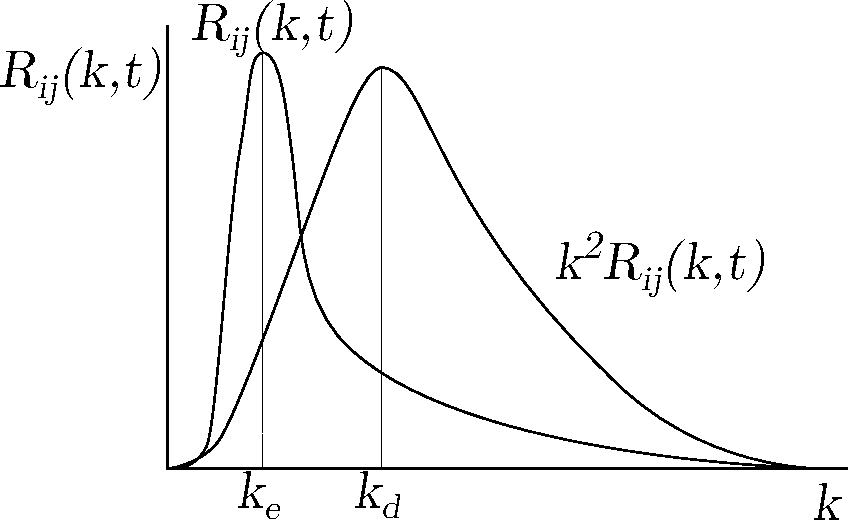
\includegraphics[width=0.6\textwidth]{clase07/energia_fourier.pdf}
\caption{Gráfico de energía con respecto a escalas de movimiento}
\label{figenergia_fourier}
\end{figure}

Aquí ocurre algo interesante: mientras la energía cinética entra al sistema por las grandes escalas (la cuchara que revuelve), la disipación de energía cinética ocurre en las pequeñas escalas.
Esto nos dice que tiene que haber un mecanismo de transferencia de energía cinética desde los vórtices grandes a los pequeños, en lo que se llama la \emph{cascada de energía}.
